\documentclass[11pt, titlepage]{article} % use larger type; default would be 10pt
\usepackage[utf8]{inputenc} % set input encoding (not needed with XeLaTeX)

%%% PAGE DIMENSIONS
\usepackage[margin=1in]{geometry}
\usepackage{setspace}
\doublespacing
%\setlength{\parskip}{2em} % setting skips between paragraphs

%%% HEADERS & FOOTERS
\usepackage{fancyhdr} % This should be set AFTER setting up the page geometry
\pagestyle{fancy} % options: empty , plain , fancy
\renewcommand{\headrulewidth}{0pt} % customise the layout...
\lhead{}\chead{}\rhead{}
\lfoot{}\cfoot{\thepage}\rfoot{}


%%% SECTION TITLE APPEARANCE
\usepackage{sectsty}
\allsectionsfont{\sffamily\mdseries\upshape} % (See the fntguide.pdf for font help)
% (This matches ConTeXt defaults)


%%% ToC APPEARANCE
\usepackage[nottoc,notlof,notlot]{tocbibind} % Put the bibliography in the ToC
\usepackage[titles,subfigure]{tocloft} % Alter the style of the Table of Contents
\renewcommand{\cftsecfont}{\rmfamily\mdseries\upshape}
\renewcommand{\cftsecpagefont}{\rmfamily\mdserfies\upshape} % No bold!


%%% BIBLIOGRAPHY
\usepackage[american]{babel}
\usepackage{csquotes}
\usepackage[backend=biber, useprefix=true, style = apa, sorting = nyt]{biblatex}
\setlength\bibitemsep{\baselineskip}
\newcommand{\mycite}[2][]{%
  (\parenciteauthor*{#2}, \parenciteyear{#2}\ifx\relax#1\relax\else:#1\fi)}


%% PACKAGES
\usepackage{verbatim} % adds environment for commenting out blocks of text & for better verbatim
\usepackage{tabularray} % for use with tinytables
\usepackage{codehigh}
\usepackage[normalem]{ulem}
\UseTblrLibrary{booktabs}
\newcommand{\tinytableTabularrayUnderline}[1]{\underline{#1}}
\newcommand{\tinytableTabularrayStrikeout}[1]{\sout{#1}}
\NewTableCommand{\tinytableDefineColor}[3]{\definecolor{#1}{#2}{#3}}
\usepackage{float} % for arranging figures
\usepackage{caption} % for figure captions 
\usepackage{subfig} % make it possible to include more than one captioned figure/table in a single float
\usepackage{graphicx} % support the \includegraphics command and options
\usepackage{ltablex} % for creating tables
\usepackage[runin]{abstract} % abstract formatting
\usepackage{enumerate} % for control over enumerated lists
\usepackage{titling} % for control over titles
\usepackage{authblk} % for including affiliations
\usepackage{booktabs}
\usepackage{rotating} % sideways figures and tables
\usepackage{placeins}
\usepackage{dcolumn}

%%% CAPTIONS AND NOTES
\captionsetup*{labelfont={bf,footnotesize},textfont={it},labelsep={period},justification=centering,singlelinecheck=false}
\captionsetup*[figure]{name=FIGURE}
\captionsetup*[table]{name=TABLE,position=top,justification=raggedright}
\newcommand{\floatnotes}[2][Notes: ]{%
  \par\medskip%
  \begingroup%
  \begin{minipage}{0.9\linewidth}
  \raggedright\footnotesize%
  \emph{#1}#2\par
  \end{minipage}\endgroup%
}


%%% ABSTRACT FORMATTING
\setlength{\abstitleskip}{-\parindent}
\abslabeldelim{\quad}
\setlength{\absleftindent}{1em}
\setlength{\absrightindent}{1em}
\preto{\abstract}{%
  {\noindent\rule{\textwidth}{1pt}}\vspace*{1em}%
}
\appto{\endabstract}{%
  \vspace*{1em}%
  {\noindent\raisebox{1em}{\rule{\textwidth}{1pt}}}\vspace*{\baselineskip}
}

\providecommand{\keywords}[1]
{
  \small	
  \textbf{\textit{Keywords---}} #1
}


% MATH WRITING
\usepackage{amsmath} 
\usepackage{amssymb}
\usepackage{ntheorem}
\newtheorem{hyp}{Hypothesis} 
\newtheorem{subhyp}{Hypothesis}
   \renewcommand\thesubhyp{\thehyp\alph{subhyp}}

%%% PATHS TO FIGURES, BIBLIO, ETC
%\graphicspath{{figures/}}
\addbibresource{paper3.bib}

\usepackage{color}
\usepackage{hyperref}
\usepackage{fontawesome5}
\definecolor{linkcol}{RGB}{34, 139, 34}
\hypersetup{colorlinks,breaklinks,
	linkcolor=linkcol,urlcolor=linkcol,
	anchorcolor=linkcol,citecolor=linkcol}
 
 
%%% Setting Font
\usepackage[bitstream-charter]{mathdesign}
\usepackage[T1]{fontenc}





%% Full title
\title{Evasive Maneuvers: The Impact of One-Sided Violence on Foreign Investment}
\author{Steven Saroka and Tyler Ditmore}
\date{\today}




\begin{document}



\newgeometry{margin=1.5in} % Adjust the margin values as needed
\begin{titlepage}


\thispagestyle{plain}


\singlespacing






\begin{center}
    \huge
    \textbf{Evasive Maneuvers: The Impact of One-Sided Violence on Foreign Investment} \\ 
         
  \vspace{1cm}
    \Large
    \textbf{Steven Saroka and Tyler Ditmore}

          \vspace{0.2cm}
    
    \vspace{0.2cm}
    \today
    
	\normalsize
 
    \vspace{1cm}
    
    \textbf{Abstract}
\end{center}

The relationship between foreign direct investment and one-sided violence (OSV) has not been studied. However, the potential impact of OSV on FDI decisions, including whether to send FDI through tax havens, deserves consideration given the role of FDI in the global economy. In this paper, we explore the connections between one-sided violence and FDI from tax havens. We argue that, should a state engage in OSV, multinational corporations will become more likely to route their investment into that state through a tax haven. They do so to maintain a level of privacy surrounding their investment, which helps them to prevent potential sanctions and other legal restrictions from their home state from interfering with their investment. This theory predicts that as a target state experiences OSV, investment inflows from tax havens should increase relative to such inflows from non-havens. We test this using newly available state-level investment data from the IMF, finding very little support for the theory from cross-national time-series regression models.


\vspace{1cm}

\keywords{FDI, One-Sided Violence, Tax Havens}

\clearpage


\end{titlepage}
\restoregeometry
\doublespacing

\section*{Introduction}

To what extent does one-sided violence (OSV) have an effect upon foreign direct investment (FDI)? Much of the existing literature on these topics has focused on either OSV or FDI, but there has been very little connection between these two areas of research. The study of OSV has primarily focused on determining its risk factors and causes, usually in the context of a state experiencing civil war \parencite{kalyvas2006logic,Weinstein07}. However, there have been almost no attempts to consider these states not just as victims of civil war or potential perpetrators of OSV, but also as potential recipients of FDI. If OSV is an action taken by FDI recipients, what impact does this action have on the behavior of FDI suppliers?

While the economic characteristics of FDI recipients have long been a subject of interest \parencite{jensen2006}, and this research contributes to that effort by considering other characteristics of FDI recipients, the characteristics of FDI senders are of vital importance as well. The home institutions of MNCs may structure their perceptions of risk in target states \parencite{beazerConditionalNaturePolitical2018}. It may also influence their appetite for corruption, and for facilitating new corruption through FDI \parencite{brazysSunshineCurseForeign2020}. The rise of new exporters of capital, especially China, may negatively affect politics in recipient countries because of the new preferences and home environments of the MNCs \parencite{yangRacingBottomChinese2023}. Given the potential consequences that home states can have upon host states' institutions, and the fundamental decay of institutions in states engaged in one-sided violence against their own citizens, this is a vital area to explore. 

Yet FDI source data can be notoriously difficult to parse. This is due to the complicated legal structures that MNCs set up in tax havens \parencite{findleyGlobalShellGames2012}. MNCs in separate countries are treated as entirely separate entities, which allows them to create shell structures that reduce their corporate tax burden without engaging in real economic activity in a country \parencite{keenCorporateTaxationGlobal2019}. The potential resource gain from changing legal rules to attract such profit shifting has contributed to the centrality of small states to international finance in ways that far outweigh their real economic importance \parencite{garcia-bernardoUncoveringOffshoreFinancial2017}. This in turn skews the nature of FDI data, as corporate tax havens like Singapore and the Netherlands are always among the top exporters of investment despite not being the largest producers of capital. Thus, any study attempting to examine the consequences of the characteristics of a host state (such as whether it is engaged in one-sided violence) upon source country FDI must first consider the importance of tax havens to international finance. 

Together, this preexisting research implies a research question — given the signals OSV can send to international investors, how do investors change their FDI activity in response to those signals? This paper provides a preliminary theoretical account of how OSV impacts FDI source country investments once tax havens are considered, based on the existing prior research. MNCs route their investments through tax havens primarily to reduce their tax burden through profit shifting. However, creating such investment structures also generates side benefits that can be leveraged in later circumstances, such as in investor-state dispute settlements \parencite{thrallSpilloverEffectsInternational2021}. One prominent externality of tax havens is secrecy. While secrecy is primarily intended to support tax avoidance, which is frequently seen as a legal-yet-negative activity, it can also be useful when investment decisions themselves will be met with opprobrium. This should especially be the case when the target or host state is engaged in one-sided violence against its citizens. Because state-perpetrated OSV  is a substantial violation of human rights, its occurrence can and sometimes does draw international condemnation, which can lead to restrictions on investment. In these particular cases, the legal privacy provided by tax havens becomes more salient for their ongoing investment operations. Thus, when MNCs have an interest in direct investment in such a state, they will be more likely to avail themselves of tax havens as part of their financial structure to obviate the impact of potential backlash.  

We predict, then, that as a target state engages in OSV, FDI originating from tax havens should increase relative to FDI originating from non-havens. We use novel data on bilateral investment stocks from the International Monetary Fund's Coordinated Direct Investment Survey (CDIS) \parencite{internationalmonetaryfundCoordinatedDirectInvestment2015}, combined with one-sided violence data from the Uppsala Conflict Data Program’s One-sided Violence Dataset version 23.1 \parencite{eck2007one,davies2023organized}.  We conduct time-series cross-sectional regressions on this data, further probing our findings by exploring the relationship between civil conflict and observations being marked as ``Confidential" in the IMF data as well as checking for multicollinearity. Our models do not provide much support for our hypothesis, but these findings are still a useful contribution to the study of MNC decision-making and political violence more broadly.


\section*{Literature Review}

There has been very little research on whether the occurrence of one-sided violence (OSV) in a state impacts whether FDI inflows to that state are sent through tax havens. While this has not been an area of focus in previous research, creating a gap this paper intends to fill, these phenomena have been studied separately. There is a growing literature on FDI and tax havens, as well as an established literature on OSV. As this literature review shows, there is little interaction between these two separate areas of research. This lack of interaction between them is something this paper’s theory aims to begin to remedy.

\subsection*{FDI and Tax Havens}

Many studies of the role of FDI in the global economy overlook a major feature of how FDI is typically conducted: through tax havens. MNCs are governed by a taxation principle which assumes that their subsidiaries in different countries operate at ``arm’s length” from each other, meaning their transactions across countries are supposed to be purely market-based \parencite{keenCorporateTaxationGlobal2019}. However, MNCs are also very clearly large, hierarchical organizations which engage in extensive planning to reduce tax burdens via those same transactions. They use the accepted norms of international taxation to register profits in jurisdictions that set lower corporate tax rates \parencite{wangCorporateTaxAvoidance2020}. These jurisdictions---which we term \textit{tax havens} but may also be referred to as offshore financial centers or secrecy jurisdictions---are hallmarked by their provision of financial services to foreign investors in scale that exceeds their real economic production \parencite{zoromeConceptOffshoreFinancial2007}. This has resulted in a plague of tax avoidance \parencite{torslovMissingProfitsNations2023} while sparking competition amongst a variety of countries to become tax havens that attract MNC profits without attracting their investments \parencite{garcia-bernardoUncoveringOffshoreFinancial2017}. Rather than generating real, productive economic activity, these countries become tax havens by effectively commercializing their sovereignty for the benefit of MNCs \parencite{palanTaxHavensCommercialization2002}. 

This material incentive for an MNC to route investments through tax havens has two primary unintended consequences on international investment beyond the obvious problem for the state of tax avoidance. First, it re-centers international legal power away from areas of genuine economic activity and towards jurisdictions where MNC profits are parked \parencite{sharmanCanariesCoalMine2012}. For instance, MNCs launch investor-state dispute settlements from tax havens frequently, which allows them to pick and choose where in their production chain they expect to have the most settlement success. This privileges tax havens with established legal regimes \parencite{thrallSpilloverEffectsInternational2021}. The legal regimes built up around tax havens to protect and attract investments become compelling motivations for financial activity in their own right: development banks park their funding in offshore accounts to protect against expropriation \parencite{carterWhyDevelopmentFinance2017}. This gives tax havens a disproportionately large legal impact on the international system.

\begin{figure}[t!]%
    \centering
       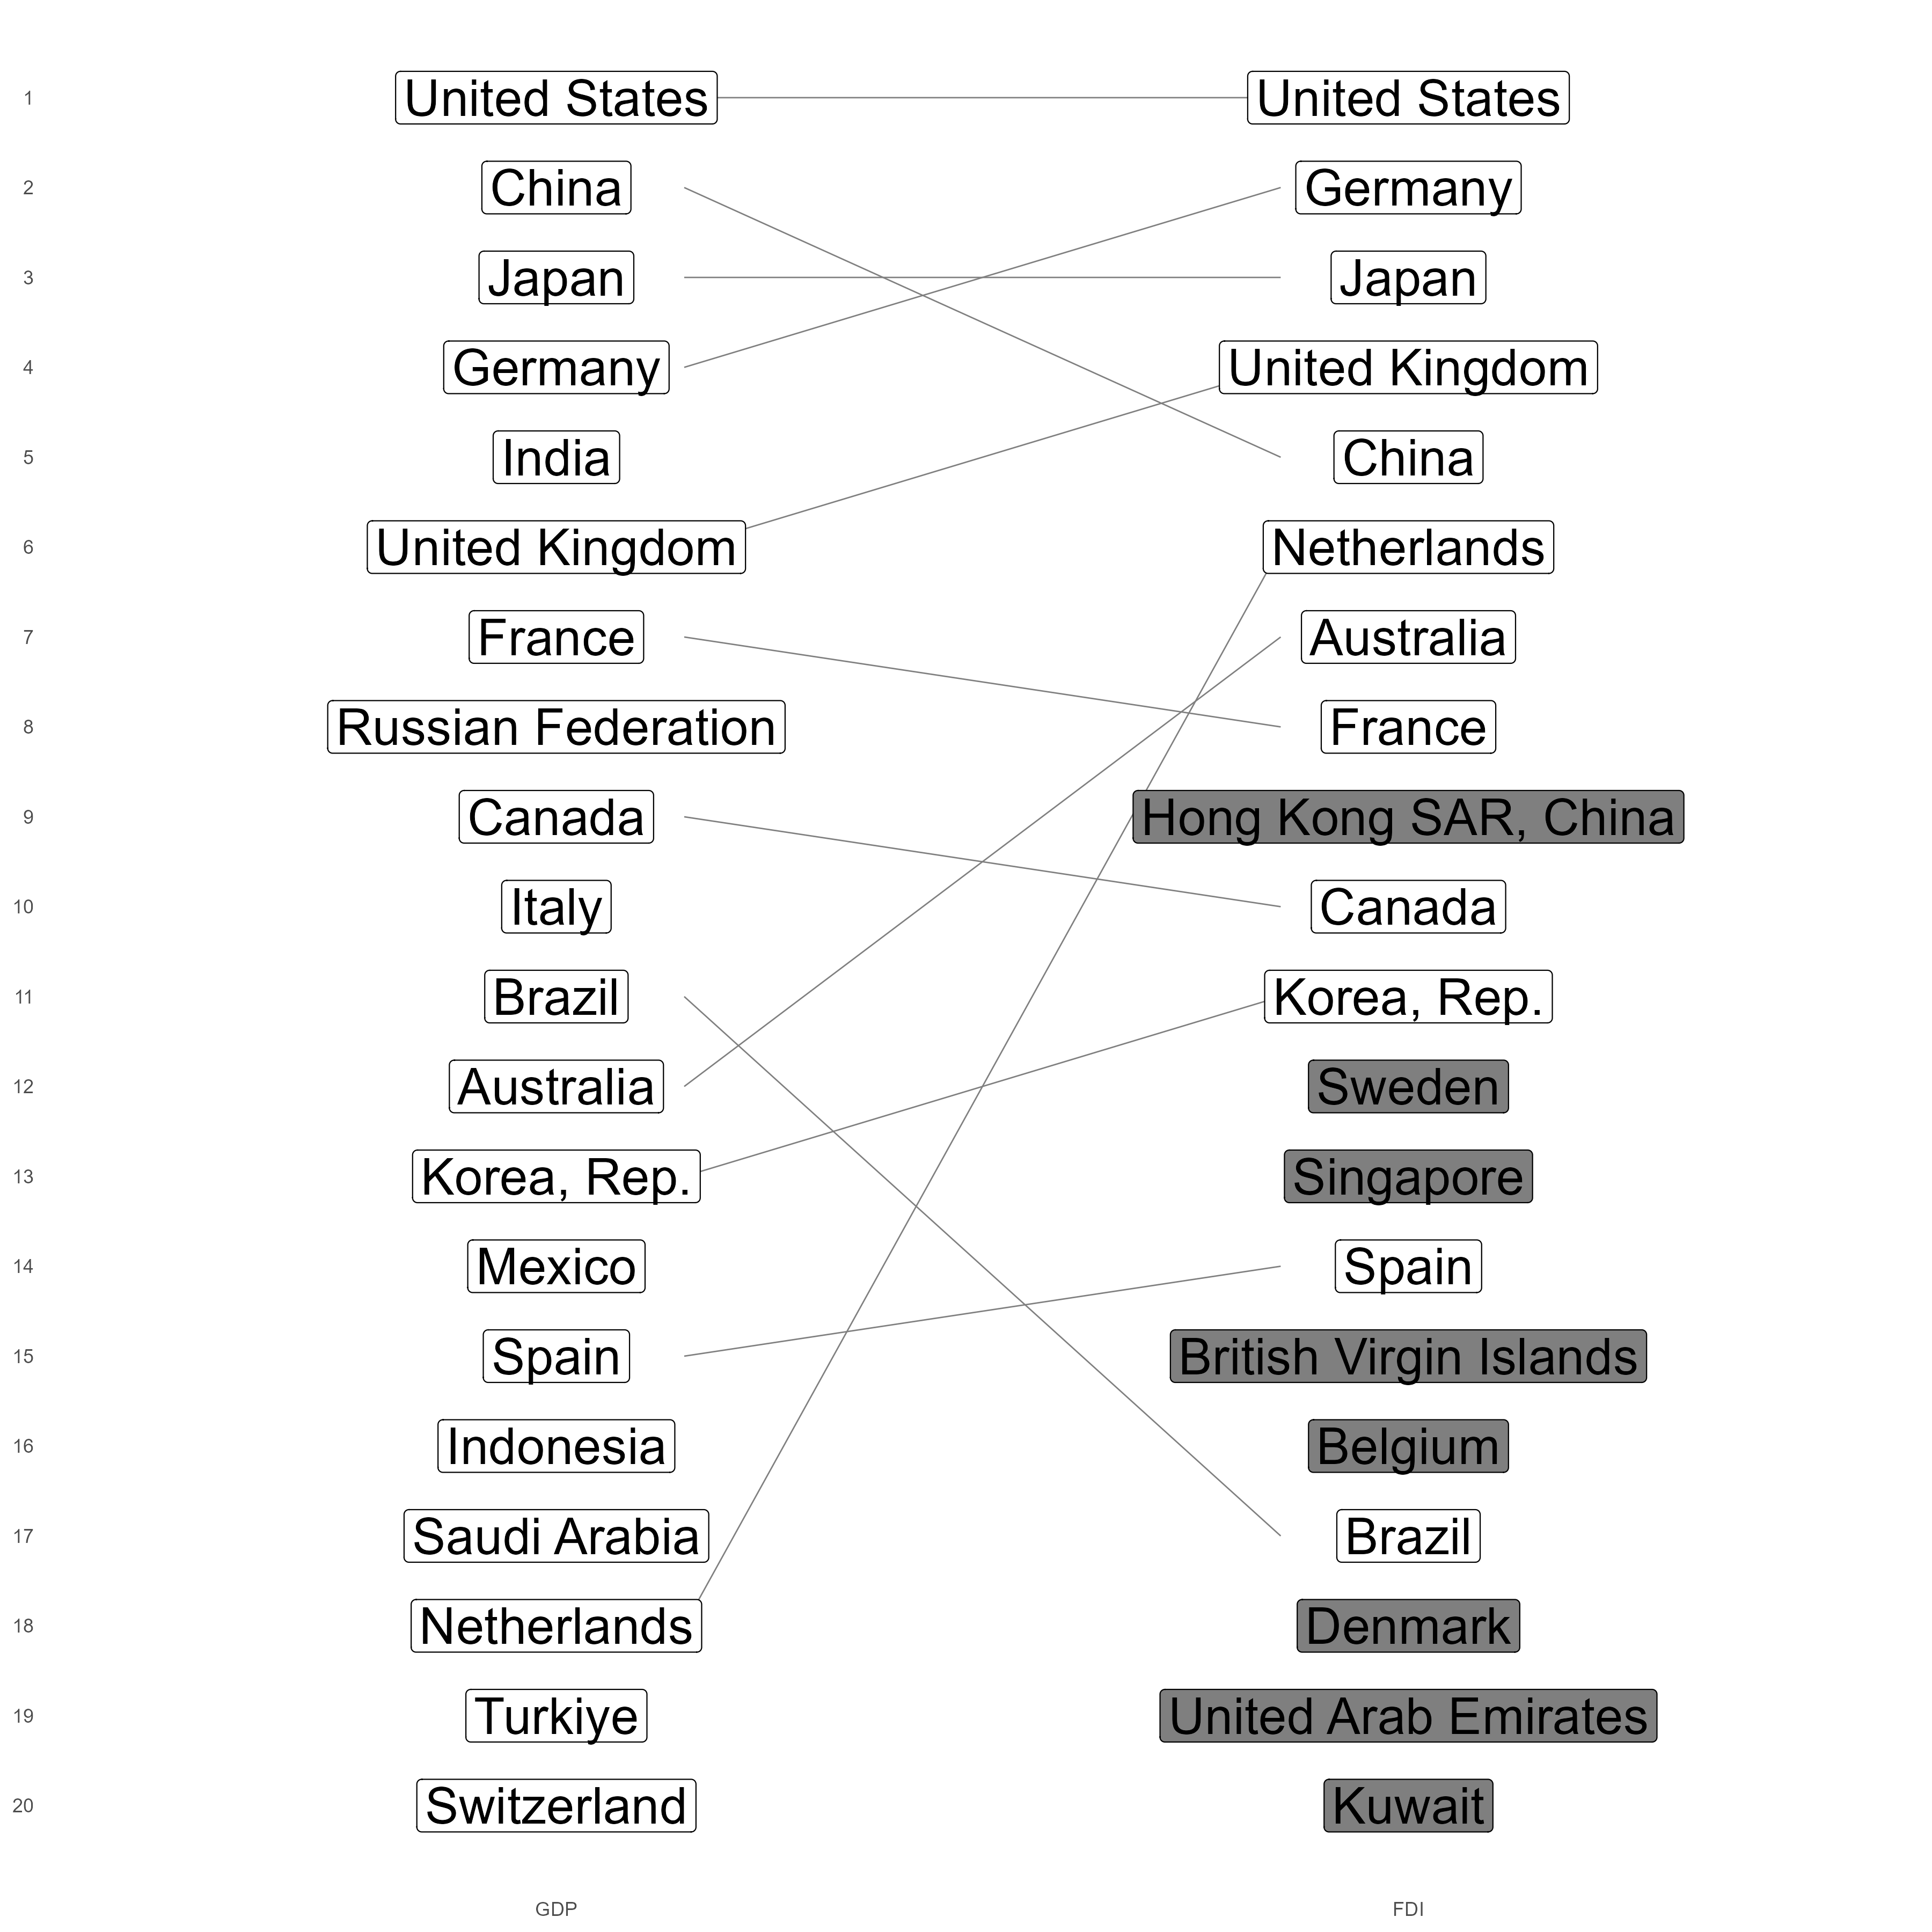
\includegraphics[width=.85\linewidth, keepaspectratio]{fdi_plot_2022.png}
\caption{World Leaders in GDP and FDI (2022)}
\floatnotes{Displays the ordered rankings of the top 20 countries by gross domestic product (current USD) and net FDI outflows (current USD) in 2022. Grayed countries in the FDI column are countries that are not in the top 20 for GDP. Data taken from the World Development Indicators.}
\label{fig:fdi_plot_2022.png}%
\end{figure}

The second consequence is that the growth of tax havens to service MNCs also facilitates international financial secrecy. Tax havens that service MNCs also facilitate the cheap creation of offshore shell companies and trusts \parencite{findleyGlobalShellGames2012}. These legal entities are in turn highly attractive to individuals who wish to hide money away from the prying eyes of corruption watchdogs and tax agencies \parencite{christensenLootingContinuesTax2011, cooleyTransnationalCorruptionGlobalized2017}. Thus, tax havens facilitate leaders stealing money from their countries’ oil revenues \parencite{andersenPetroRentsPolitical2017} and capturing personal rents from foreign aid \parencite{andersenEliteCaptureForeign2020}. 

The importance of these developments can be seen in Figure \ref{fig:fdi_plot_2022.png}, which displays the top 20 countries by GDP and FDI outflows for 2022. If FDI outflows are connected to the surplus capital in a country, then they should also be highly related to GDP. We do see this for the overall richest countries, such as the United States and China. However, we also see that the top FDI exporters include much smaller countries and jurisdictions, including Hong Kong, Singapore, and Belgium, which are known to be offshore financial centers. We also see the disproportionately high rank of countries like the Netherlands, which hosts a notorious corporate tax avoidance scheme. On the other side, massive economies like India and Indonesia do not register as top FDI exporters. 

Tax havens are important intermediaries of FDI, then, but we know very little about how they play a role in investments into states engaged in any kind of violence, including in one-sided violence against their populations. However, one-sided violence has been studied separately, as covered in the next section. 

\subsection*{One-Sided Violence}

The topic of one-sided violence (OSV), broadly defined as the intentional killing of civilians by governments and non-state actors \parencite{fjelde2021introducing},\footnote{This definition also agrees with the definition used in the Uppsala Conflict Data Program’s One-sided Violence Dataset version 23.1 \parencite{eck2007one,davies2023organized}, where OSV is defined as "the use of armed force by the government of a state or by a formally organized group against civilians which results in at least 25 deaths" (3) in a year \parencite{pettersson2023codebook}.}  has been a focus of conflict scholarship for some time. Much of this scholarship has focused on the role of OSV in civil wars, guided by the initial influence of research such as \textcite{kalyvas2006logic} and \textcite{Weinstein07}. This research into OSV has produced many useful findings, but faces a reversed problem compared to the FDI literature cited above, as it has not expanded to seriously consider how this violence may impact international financial flows.

It is well-established that both rebels and the state can engage in one-sided violence against civilians, with the levels and direction of violence frequently depending on shifting power dynamics between the state and the rebel group(s) \parencite{kalyvas2006logic,kalyvas2007free,wood2012armed}. While this violence can vary by whether it is selective, collective, or indiscriminate \parencite{kalyvas2007free,schubiger2023one}, the exact label of the violence matters less for the purposes of our theory than its occurrence. Whether states and rebels engage in OSV depends on several factors. Mass killing can be a strategy deliberately chosen by the state to remove rebel support \parencite{valentino2004draining, downes2007draining}, or an incidental byproduct of the starting resource endowments of a rebellion \parencite{Weinstein07}. It can be driven by both preexisting political divisions and dynamics endogenous to the conflict itself \parencite{ balcells2010rivalry}. Strategic considerations of how domestic and international audiences will respond to its occurrence can also influence whether rebels and states engage in OSV \parencite{stanton2016violence}. While this literature has covered a wide range of factors contributing to OSV's occurrence, the role (if any) played by FDI has not yet been considered.

The actual amount and effectiveness of violence committed against civilians can also vary by several factors, including the extent of local support for rebels \parencite{toft2015islamists, zhukov2017external} and how far the targets of repression are from the center of the state’s ability to project power \parencite{cunningham2009takes}. From the perspective of the state, the effectiveness of one-sided violence may be dependent on its amount: extreme repressive violence prevents an opposition from recruiting and continuing to oppose the state, while low or moderate repressive violence fails to do so \parencite{zhukov2023repression}. States attempting to use one-sided violence to prevent the occurrence of civil war may find these attempts backfire, as the occurrence of OSV is a risk factor for civil war onset \parencite{ young2013repression, cederman2020civilian}. Again, these factors are exclusively non-economic in nature, pointing to the need for more consideration of whether economic factors such as FDI influence these occurrences.

Despite its depth, this literature rarely considers economic factors, including whether instances of OSV may impact current or future FDI. This is somewhat puzzling, as OSV has frequently been studied in the context of civil wars, and there is a fairly robust literature on the relationship between civil wars and FDI. While that literature covers FDI and civil war onset \parencite{bussmann2007globalization, sorens2014globalisation, mihalache2018whose}, FDI during civil wars \parencite{Asiedu2006,jensen2006,jensenyoung2008,bussmann2010,livashchilko2010, Wittetal2017, OhOetzel2017,barry2018}, and FDI during post-conflict recovery \parencite{allee2010, billing2019,bak2021intrastate}, both the role of tax havens in FDI and the potential impact of OSV on such FDI is not explored. Aside from one study that found that FDI inflows may motivate one-sided violence by governments of developing states, if those states were experiencing lower civil liberties respect or unhealthy economic situations \parencite{kishi2017foreign}, this literature is characterized by a lack of consideration of how economic factors such as FDI may influence or be influenced by OSV. 

\subsection*{Review Conclusion}

This review of the literature on FDI, tax havens, and OSV shows that scholars have researched these topics separately, and sometimes researched two of them together, but have never considered whether all three are linked. This literature offers a few hints on what such a linkage would look like. One starting point is the legal and jurisdictional benefits of sending investments through tax havens. These are likely to extend to investments into states engaging in a variety of activities that the international community may find unsavory, including committing violence against their own civilians. This implies a question: to what extent does the existence of tax havens as financial intermediaries of legal privilege and jurisdictional secrecy mediate the way FDI is affected by the occurrence of OSV? We attempt to answer this with our theory.


\section*{Theory}

How does OSV impact the choices made by senders of FDI? In particular, why would a multinational corporation opt to route FDI going into states where the government is committing one-sided violence against the civilian population through a tax haven, rather than investing directly in the target state? Answering this question requires first establishing a general logic of why MNCs use tax havens, regardless of the characteristics of the eventual target of their investment.

By virtue of the obsolescing bargain, MNCs have sufficient negotiating leverage to extract favorable tax provisions upon entry into a country \parencite{ramamurtiObsolescingBargainingModel2001, hauflerCountrySizeTax1999}. A state engaging in one-sided violence, especially if it also experiencing ongoing civil conflict,\footnote{While the phenomena of OSV and civil conflict are theoretically distinct occurrences, they are also linked by a tendency to co-occur, with OSV being a frequently-studied element of civil conflict theorized to be influenced by shifting power dynamics between the state and rebel group(s) \parencite{kalyvas2006logic,wood2012armed}. While our theory focuses on OSV, this overlap is unavoidable both theoretically and empirically, as all OSV in our timeframe (see Methods) occurs during instances of civil war. Thus, while the scope of this theory is limited to states receiving FDI while their government is engaging in OSV, the context of civil war is an unavoidable backdrop.} is unlikely to be able to afford to scare off investors by not acceding to such demands or by threatening to extract new rents from the investment after it is in place. Sending investment from an MNC’s home state through a tax haven to its eventual destination (host) state would, on its face, appear to be an extra level of potentially expensive and time-consuming complication for the business.

In line with established literature, we posit that MNCs take on the extra complication of routing investment through tax havens for the primary purpose of securing tax privileges for their investments. Tax havens allow corporations to legally avoid taxes, which has been widely acknowledged for decades \parencite{bartelsmanWhyPayMore2003}. Moreover, tax avoidance has long been facilitated and encouraged by wealthy economies to give their corporations a competitive advantage \parencite{hakelbergHypocriticalHegemon2020}. This creates legal and material incentives for MNCs to develop investment structures based in or routed through tax havens, regardless of the final destination of their investment.

Once the tax haven investment structure becomes entrenched in MNC planning, it generates spillover effects \parencite{thrallSpilloverEffectsInternational2021}. Tax havens market privacy for individuals, which allows corrupt officials to stash away the gains from graft into offshore financial institutions \parencite{christensenLootingContinuesTax2011}. While MNCs can quite publicly avoid tax payments due to the legal privileges of tax havens, and thus do not require secrecy for their investments in havens, the legal secrecy that havens can afford offers them additional privacy in instances of controversial investment decisions. It is this feature of tax havens that makes them especially relevant in certain cases where the target state for FDI is also engaging in one-sided violence against civilians.

This theory's scope is limited to states where one-sided violence (OSV) is committed by the government of the target state against civilians within that state. We specifically focus on government actions because state governments are the only actors with the internationally recognized legal authority to allow or stop FDI ventures within their territory. While other actors (like rebel or terrorist groups) can also engage in OSV, they generally lack the international legitimacy accorded to the state, as well as the ability to deny FDI entrance to the entire state (even if rebels can attempt to make FDI ventures in specific areas prohibitively dangerous). 

Because of the importance of the state to prospective FDI inflows, the occurrence of state OSV adds an additional dimension to MNC decisions to engage in FDI in a state committing it. Because state-perpetrated OSV is a substantial violation of human rights, its occurrence can and sometimes does draw international condemnation, which can lead to restrictions on investment.\footnote{While not sharing our specific theoretical focus on OSV, \textcite{murdie2013impact} provides evidence for a linkage between international condemnation from human rights organizations and economic sanctions.} In these particular cases, the legal privacy provided by tax havens becomes more salient for their ongoing investment operations.

In the case of states with governments committing OSV, which have the potential to attract international condemnation (even if it does not always occur), sending FDI through a tax haven enables a corporation to avoid meaningful impacts to their operations. In addition to the standard benefits to the corporation in the form of lower effective tax rates on profits from their investment, this use of tax havens allows MNCs to mitigate the impacts of any economic measures taken by their home state against the target state due to international condemnation. Should an MNC's home state respond to reports of OSV with trade embargoes or sanctions, for example, using a tax haven may allow that multinational corporation to begin a new investment or continue extracting profits from its pre-existing investment without state interference. Additionally, such economic punishments need not even be realized for this logic to guide MNC behavior. MNCs can use the protective shelter of a tax haven as a preemptive shield against the future threat of lost profits, even if their home state has yet to take action in response to international condemnation. Thus, we expect that tax havens will become more attractive elements of investment plans into states committing OSV, leading to more investment inflows being routed through tax havens on their way to the target state compared to investment inflows that do not involve tax havens.


\begin{hyp}
    As a target state engages in government-perpetrated OSV, investment inflows from tax havens should increase relative to inflows from non-havens.
\end{hyp}

This hypothesis is phrased in relative terms (inflows from havens versus inflows from non-havens) rather than absolute terms due to the focus of the theory on relative differences in FDI from different origin points. The absolute amount of FDI coming from a given tax haven or non-haven is less theoretically salient than whether more FDI originates from a haven or non-haven. As we are interested primarily in changes in the amount of FDI coming from two different origin points, and whether one of those origin points becomes more common relative to the other, focusing on relative rather than absolute amounts of FDI makes more theoretical sense. 


\section*{Research Design}

\subsection*{FDI Data}

Historically, researchers have been limited by the aggregate nature of FDI data in terms of exploring more fine-grained distributional effects of violence on international investment. We offer one means of redressing this by using the relatively recent publication of the IMF's Coordinated Direct Investment Survey (CDIS) \parencite{internationalmonetaryfundCoordinatedDirectInvestment2015}. The IMF began collecting the CDIS in 2009 in an effort to disaggregate direct investment by recipient and sender. It requires participating countries to survey firms and tabulate both foreign ownership of domestic firms and domestic ownership of foreign firms. They then group the data together and report direct investment stocks to the IMF, separated by type of investment and by investment counter-party. It is thus the best widely-available, public bilateral FDI data, and has been used to estimate international tax avoidance \parencite{janskyPanamaReallyYour2021} and examine how political ties between dyads affect financial flows \parencite{beazerConditionalNaturePolitical2018}. 

Although reporting to the IMF is voluntary, coverage is broad and is markedly better than firm-level data for gathering information on developing countries. Between 92 and 122 countries have reported every year since 2009, including up to 21 states labeled as tax havens according to a 2007 IMF definition of offshore financial centers \parencite{zoromeConceptOffshoreFinancial2007}.\footnote{Note that we use this base list but add the Netherlands, as it had yet to be labeled a tax haven in 2007 but is now considered a major MNC tax sanctuary; this follows procedures conducted elsewhere in examining corporate tax avoidance \parencite{torslovMissingProfitsNations2023}. A list of these states, and the years during which they reported data to the CDIS, can be found in Table \ref{tab:popSubcomp}.} Because these reporters come from the largest economies and report on the FDI stock held in other countries, they end up with near-universal coverage of FDI hosts: 242 total states and territories. This affords us coverage of FDI into developing countries that are experiencing one-sided violence, which is otherwise hard to gather. 

Even so, the data remains a patchwork. Among other things, countries are allowed to suppress public data as `Confidential' for fear of revealing details that could be used to identify surveyed firms. This is more likely to happen in cases where investment amounts are small or when investment locations are sensitive, which, per our theory, is likely the case. As such, we expect that there may be under-reporting in the data of FDI flowing into these states, and these results will represent a lower bound estimate. In spite of the potential pitfalls of the data, it remains the best option for empirically examining our theory via a large-N quantitative analysis of the IMF CDIS data. We discuss the specific models we use in the next section.  

\subsection*{Quantitative Analysis Variables and Models}

Throughout this analysis, the unit of analysis is the country-year, and the timeframe of this analysis is the years 2009-2019. The CDIS data starts in 2009, and years post-2019 are excluded to avoid the impact of the COVID-19 pandemic on international trade and investment from biasing the analysis. 

The dyadic nature of the data allows us to break apart FDI stocks in an economy by their source, specifically by whether or not the owner comes from a tax haven. We use \textit{Net Inward Direct Investment Positions}, broken down by year and dyad. We denote whether or not the FDI stock has its origin from a tax haven, using a 2007 IMF definition of offshore financial centers \parencite{zoromeConceptOffshoreFinancial2007}.\footnote{FDI stock is the total collected amount of direct investment reported in a country. FDI flows are the changes in FDI stock from year to year. We use FDI stocks, as reported by the CDIS, throughout this study.} We use this definition for two reasons. First, it is a largely political definition of tax havens that was developed by the IMF prior to the institution of the CDIS data series, and thus any change by tax havens as a result of being labelled as such should occur before this series began. Second, it has been used in other studies to indicate tax haven investment \parencite{andersenEliteCaptureForeign2020}, and thus our analysis matches the prevailing norm. 

Our first dependent variable is \textit{Relative FDI Tax Haven Share}. For each investee country, we divide the reported net FDI stock in a given year into that sourced from tax havens and that sourced from non-havens. We standardize both by the state's GDP in current USD, to enable comparability across years. We then divide the tax haven amount by the sum of both tax haven and non-haven amounts to create a measure of the share of tax haven FDI present in a given country-year. Figure \ref{fig:dv1histo} displays a histogram of this dependent variable, showing a substantial right skew centered around .5. There are some limited positive and negative outliers, due to the fact that 51 net FDI stock values were negative, but the vast majority of these values were positive.\footnote{This relative share variable is itself a ratio of ratios, given that FDI stocks are a balance of investment into and out of a state by a firm.} 

	\begin{figure}
    \centering
		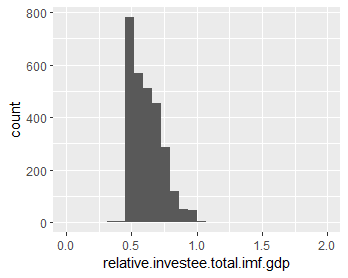
\includegraphics[scale=1]{dv1histo.png}
		\caption{Histogram of Relative Tax Haven Share Variable. Variable shown is the relative amount of investment from tax havens, calculated as the total investment inflows from all tax havens divided by the total investment inflows from all sources.}
		\label{fig:dv1histo}
	\end{figure}

As shown in \ref{fig:dv1histo}, this data is not normally distributed. Given this, we specify three additional dependent variables: logged total tax haven FDI stocks, logged total non-haven FDI stocks, and logged total FDI stocks.\footnote{This led to the exclusion of 51 observations with negative stock values from analyses using these variables.} As shown in Figures \ref{dv2histo}, \ref{dv3histo}, and \ref{dv4histo}, logging produces a distribution that looks much more normal.

	\begin{figure}
 \centering
		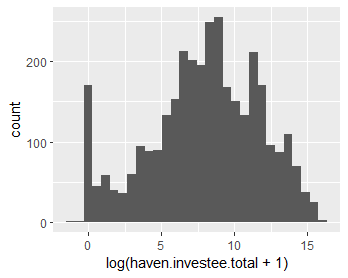
\includegraphics[scale=1]{dv2histo.png}
		\caption{Histogram of Logged Tax Haven FDI Stocks. The dependent variable shown here is only composed of FDI stocks originating from tax havens.}
		\label{dv2histo}
	\end{figure}

	\begin{figure}
 \centering
		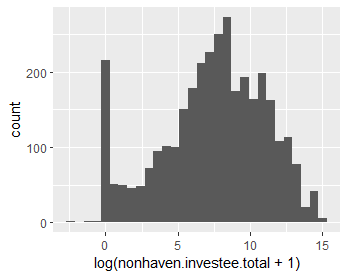
\includegraphics[scale=1]{dv3histo.png}
		\caption{Histogram of Logged Total Non-Haven FDI Stocks. The dependent variable shown here is only composed of FDI stocks originating from non-haven investor states.}
		\label{dv3histo}
	\end{figure}

	\begin{figure}
 \centering
		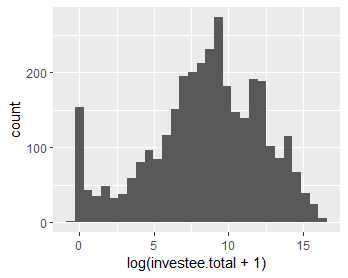
\includegraphics[scale=1]{dv4histo.png}
		\caption{Histogram of Logged Total FDI Stocks. The dependent variable shown here is composed of FDI stocks originating from all investor states.}
		\label{dv4histo}
	\end{figure}

Data on one-sided violence comes from the Uppsala Conflict Data Program’s One-sided Violence Dataset version 23.1 \parencite{eck2007one,davies2023organized}. They define OSV as "the use of armed force by the government of a state or by a formally organized group against civilians which results in at least 25 deaths" in a year \parencite{pettersson2023codebook}, which fits well with the definitions of OSV given in the literature above. We filter the data to only contain OSV committed by state actors, leaving us with 118 country-years of OSV in our data. The amount of casualties varied substantially across country-years with a mean of 232 deaths per incident of OSV but a standard deviation of 504. While the relatively low number of country-years with OSV is unfortunate, it is perhaps unsurprising given the time limitations of the FDI data. Additionally, it helps to serve as a harder test of our hypothesis, as any significant results will be more remarkable given the relative rarity of state OSV.

We incorporate several controls to help account for additional explanations that result from violence not being randomly assigned to states. To account for the impact of civil wars on FDI, we control for civil wars using data on both internationalized and non-internationalized civil conflicts from the Uppsala Conflict Data Program’s Armed Conflict Dataset version 23.1 \parencite{davies2023organized, gleditsch2002armed}. To account for the likelihood that poorer countries are more at risk for violence, we control for \textit{GDP per capita} and \textit{annual GDP growth}. To account for the potential capacity of the government as a draw for FDI, we control for \textit{natural resource rents}. To account for general country-level interest in and commitment to globalization, we control for \textit{international trade}. Furthermore, to account for larger populations being more likely to have disaffected elements be targeted by OSV, we control for \textit{population}. All of these covariates are taken from the World Bank's World Development Indicators \parencite{worldbankWorldDevelopmentIndicators2024}. We also control for the impact of regime type on FDI through the inclusion of V-Dem scores \parencite{vdem2023, pemstein2018v}. Finally, to account for time- and region-dependent dynamics, we include fixed effects for both region and year.

\section*{Results}

Here we discuss the results of regressions using the dependent variables discussed above. While the dependent variables vary across tables, with each table showing the results for a model using one of the dependent variables, the independent variables are consistent throughout all four tables. All independent variables are lagged by one year, to account for the delayed impact of information from the independent variables on investor decision-making. In all models, the lagged state OSV indicator variable is the primary independent variable of interest, taking a value of 1 if the state receiving investment was experiencing one-sided violence committed by its government during that year, and a value of 0 otherwise. All other variables are control variables for a variety of economic and political factors. 

For all models in Table \ref{relhavenDV}, the dependent variable is the relative amount of investment from tax havens, calculated as the net total investment inflows from all tax havens divided by the net total investment inflows from all sources. The first model is a naive linear regression, testing for the existence of a statistically significant association between state OSV and tax haven investment inflows in the absence of any control variables. Model 2, which adds region and year fixed effects, shows that the negative direction and non-significance of the relationship remains after adding those fixed effects. Model 3 adds the control variables discussed above, which have no impact on the direction or significance of the association. Model 4 adds the region and year fixed effects to the specification of model 3, where they make no meaningful difference. 

These results provide no evidence for our hypothesis. The coefficient is negatively signed in all models, which is not as predicted, and is also never significant. Additionally, even if these coefficients were all significant, none of them are signed in the expected direction.

\begin{table}[!htbp] \centering 
  \caption{Regression Results with Relative Haven Investment Inflows as DV} 
  \label{relhavenDV} 
\small 
\begin{tabular}{@{\extracolsep{5pt}}lcccc} 
\\[-1.8ex]\hline 
\hline \\[-1.8ex] 
 & \multicolumn{4}{c}{\textit{Dependent variable:}} \\ 
\cline{2-5} 
\\[-1.8ex] & \multicolumn{4}{c}{Relative Haven Investment Inflows} \\ 
\\[-1.8ex] & (1) & (2) & (3) & (4)\\ 
\hline \\[-1.8ex] 
 Lagged State OSV Indicator & $-$0.005 & $-$0.032 & $-$0.026 & $-$0.055 \\ 
  & (0.022) & (0.022) & (0.029) & (0.029) \\ 
  & & & & \\ 
 Lagged Civil Conflict Indicator &  &  & 0.027 & 0.019 \\ 
  &  &  & (0.014) & (0.014) \\ 
  & & & & \\ 
 Lagged GDP Per Capita (Constant 2015 Dollars) &  &  & 0.00000$^{*}$ & 0.00000$^{*}$ \\ 
  &  &  & (0.00000) & (0.00000) \\ 
  & & & & \\ 
 Lagged Annual GDP Growth Percentage &  &  & 0.0004 & $-$0.0002 \\ 
  &  &  & (0.001) & (0.001) \\ 
  & & & & \\ 
 Lagged Population &  &  & 0.000$^{*}$ & 0.000$^{*}$ \\ 
  &  &  & (0.000) & (0.000) \\ 
  & & & & \\ 
 Lagged Trade as Percentage of GDP &  &  & 0.00002 & 0.00004 \\ 
  &  &  & (0.0001) & (0.0001) \\ 
  & & & & \\ 
 Lagged Natural Resource Rents as Percentage of GDP &  &  & $-$0.0004 & $-$0.001 \\ 
  &  &  & (0.0005) & (0.001) \\ 
  & & & & \\ 
 Lagged Electoral Democracy Index &  &  & $-$0.158 & $-$0.104 \\ 
  &  &  & (0.107) & (0.113) \\ 
  & & & & \\ 
 Lagged Liberal Democracy Index &  &  & $-$0.464$^{*}$ & $-$0.428$^{*}$ \\ 
  &  &  & (0.117) & (0.118) \\ 
  & & & & \\ 
 Lagged Participatory Democracy Index &  &  & 0.494$^{*}$ & 0.534$^{*}$ \\ 
  &  &  & (0.097) & (0.098) \\ 
  & & & & \\ 
 Lagged Deliberative Democracy Index &  &  & 0.258$^{*}$ & 0.243$^{*}$ \\ 
  &  &  & (0.101) & (0.107) \\ 
  & & & & \\ 
 Lagged Egalitarian Democracy Index &  &  & $-$0.007 & $-$0.113 \\ 
  &  &  & (0.086) & (0.095) \\ 
  & & & & \\ 
 Constant & 0.623$^{*}$ & 0.554$^{*}$ & 0.609$^{*}$ & 0.534$^{*}$ \\ 
  & (0.004) & (0.014) & (0.020) & (0.027) \\ 
  & & & & \\ 
\hline \\[-1.8ex] 
Observations & 2,045 & 2,045 & 1,534 & 1,534 \\ 
R$^{2}$ & 0.00003 & 0.044 & 0.066 & 0.106 \\ 
Adjusted R$^{2}$ & $-$0.0005 & 0.037 & 0.059 & 0.090 \\ 
\hline 
\hline \\[-1.8ex] 
\textit{Note:}  & \multicolumn{4}{r}{* p<0.05} \\ 
\end{tabular} 
\end{table} 

As an alternative means of testing our theory, we separate out FDI stocks originating in non-tax haven states and tax haven states, and run the previous models again with the logged values of these as dependent variables. Given our theory, we would expect state OSV to have a positive relationship with FDI stocks from tax havens, but a negative relationship with FDI stocks from non-tax havens. Dividing our data in this way addresses the possibility that the relative investment amount variable somehow masks the effects of FDI stocks from these different sources.

First, we repeat this analysis using only logged FDI stocks originating from tax havens as a dependent variable. All other variables are the same as in the first set of models. The results are shown in table \ref{havenFDIstocksDV}, and provide no meaningful amount of support for our hypothesis. Our theory would predict a positive and significant impact of state OSV on incoming FDI stocks from tax havens, and while the two models with full controls do show a positive sign for the OSV variable, it is not significant. Additionally, the effect sizes are so small as to be effectively non-existent.

\begin{table}[!htbp] \centering 
  \caption{Regression Results with Haven FDI Stocks as DV} 
  \label{havenFDIstocksDV} 
\small 
\begin{tabular}{@{\extracolsep{5pt}}lcccc} 
\\[-1.8ex]\hline 
\hline \\[-1.8ex] 
 & \multicolumn{4}{c}{\textit{Dependent variable:}} \\ 
\cline{2-5} 
\\[-1.8ex] & \multicolumn{4}{c}{Logged Haven FDI Stocks} \\ 
\\[-1.8ex] & (1) & (2) & (3) & (4)\\ 
\hline \\[-1.8ex] 
 Lagged State OSV Indicator & $-$0.0000024 & $-$0.0000006 & 0.0000007 & 0.0000004 \\ 
  & (0.0000019) & (0.0000018) & (0.0000006) & (0.0000006) \\ 
  & & & & \\ 
 Lagged Civil Conflict Indicator &  &  & 0.0000003 & 0.0000006$^{*}$ \\ 
  &  &  & (0.0000003) & (0.0000003) \\ 
  & & & & \\ 
 Lagged GDP Per Capita (Constant 2015 Dollars) &  &  & 0.0000000$^{*}$ & 0.0000000$^{*}$ \\ 
  &  &  & (0.0000000) & (0.0000000) \\ 
  & & & & \\ 
 Lagged Annual GDP Growth Percentage &  &  & $-$0.0000000 & $-$0.0000000 \\ 
  &  &  & (0.00000002) & (0.00000002) \\ 
  & & & & \\ 
 Lagged Population &  &  & 0.0000000 & 0.0000000 \\ 
  &  &  & (0.0000000) & (0.0000000) \\ 
  & & & & \\ 
 Lagged Trade as Percentage of GDP &  &  & 0.00000002$^{*}$ & 0.00000002$^{*}$ \\ 
  &  &  & (0.0000000) & (0.0000000) \\ 
  & & & & \\ 
 Lagged Natural Resource Rents as Percentage of GDP &  &  & $-$0.00000002$^{*}$ & $-$0.00000002 \\ 
  &  &  & (0.0000000) & (0.0000000) \\ 
  & & & & \\ 
 Lagged Electoral Democracy Index &  &  & 0.0000162$^{*}$ & 0.0000127$^{*}$ \\ 
  &  &  & (0.0000023) & (0.0000024) \\ 
  & & & & \\ 
 Lagged Liberal Democracy Index &  &  & $-$0.0000163$^{*}$ & $-$0.0000127$^{*}$ \\ 
  &  &  & (0.0000025) & (0.0000025) \\ 
  & & & & \\ 
 Lagged Participatory Democracy Index &  &  & $-$0.0000074$^{*}$ & $-$0.0000091$^{*}$ \\ 
  &  &  & (0.0000021) & (0.0000021) \\ 
  & & & & \\ 
 Lagged Deliberative Democracy Index &  &  & 0.0000065$^{*}$ & 0.0000066$^{*}$ \\ 
  &  &  & (0.0000022) & (0.0000023) \\ 
  & & & & \\ 
 Lagged Egalitarian Democracy Index &  &  & $-$0.0000005 & 0.0000001 \\ 
  &  &  & (0.0000018) & (0.0000020) \\ 
  & & & & \\ 
 Constant & 0.0000025$^{*}$ & 0.0000004 & $-$0.0000039$^{*}$ & $-$0.0000055$^{*}$ \\ 
  & (0.0000003) & (0.0000012) & (0.0000004) & (0.0000006) \\ 
  & & & & \\ 
\hline \\[-1.8ex] 
Observations & 2,058 & 2,058 & 1,541 & 1,541 \\ 
R$^{2}$ & 0.0007793 & 0.1393348 & 0.3054316 & 0.3359103 \\ 
Adjusted R$^{2}$ & 0.0002933 & 0.1325878 & 0.2999769 & 0.3240594 \\ 
\hline 
\hline \\[-1.8ex] 
\textit{Note:}  & \multicolumn{4}{r}{* p<0.05} \\ 
\end{tabular} 
\end{table} 

We then run the same set of models in table \ref{nonhavenstockDV}, except with logged FDI stocks originating from non-havens. According to our theory, state OSV would be expected to have a negative impact on these FDI stocks. In line with our theoretical expectations, the OSV indicator is negative in all models, and significant in model 3. 

\begin{table}[!htbp] \centering 
  \caption{Regression Results with FDI Stocks from Non-Havens as DV} 
  \label{nonhavenstockDV} 
\small 
\begin{tabular}{@{\extracolsep{5pt}}lcccc} 
\\[-1.8ex]\hline 
\hline \\[-1.8ex] 
 & \multicolumn{4}{c}{\textit{Dependent variable:}} \\ 
\cline{2-5} 
\\[-1.8ex] & \multicolumn{4}{c}{Logged FDI Stocks from Non-Havens} \\ 
\\[-1.8ex] & (1) & (2) & (3) & (4)\\ 
\hline \\[-1.8ex] 
 Lagged State OSV Indicator & $-$0.470 & 0.076 & $-$0.999$^{*}$ & $-$0.438 \\ 
  & (0.484) & (0.383) & (0.364) & (0.336) \\ 
  & & & & \\ 
 Lagged Civil Conflict Indicator &  &  & 0.700$^{*}$ & 0.718$^{*}$ \\ 
  &  &  & (0.171) & (0.160) \\ 
  & & & & \\ 
 Lagged GDP Per Capita (Constant 2015 Dollars) &  &  & 0.0001$^{*}$ & 0.0001$^{*}$ \\ 
  &  &  & (0.00000) & (0.00000) \\ 
  & & & & \\ 
 Lagged Annual GDP Growth Percentage &  &  & $-$0.015 & 0.0003 \\ 
  &  &  & (0.011) & (0.010) \\ 
  & & & & \\ 
 Lagged Population &  &  & 0.000$^{*}$ & 0.000$^{*}$ \\ 
  &  &  & (0.000) & (0.000) \\ 
  & & & & \\ 
 Lagged Trade as Percentage of GDP &  &  & 0.004$^{*}$ & 0.003$^{*}$ \\ 
  &  &  & (0.001) & (0.001) \\ 
  & & & & \\ 
 Lagged Natural Resource Rents as Percentage of GDP &  &  & $-$0.012$^{*}$ & $-$0.003 \\ 
  &  &  & (0.006) & (0.006) \\ 
  & & & & \\ 
 Lagged Electoral Democracy Index &  &  & 0.062 & 0.744 \\ 
  &  &  & (1.319) & (1.288) \\ 
  & & & & \\ 
 Lagged Liberal Democracy Index &  &  & 5.709$^{*}$ & 4.865$^{*}$ \\ 
  &  &  & (1.436) & (1.331) \\ 
  & & & & \\ 
 Lagged Participatory Democracy Index &  &  & $-$0.358 & $-$3.092$^{*}$ \\ 
  &  &  & (1.177) & (1.096) \\ 
  & & & & \\ 
 Lagged Deliberative Democracy Index &  &  & $-$2.364 & 1.395 \\ 
  &  &  & (1.229) & (1.199) \\ 
  & & & & \\ 
 Lagged Egalitarian Democracy Index &  &  & $-$0.471 & $-$2.463$^{*}$ \\ 
  &  &  & (1.039) & (1.060) \\ 
  & & & & \\ 
 Constant & 7.376$^{*}$ & 6.626$^{*}$ & 6.075$^{*}$ & 6.291$^{*}$ \\ 
  & (0.076) & (0.238) & (0.240) & (0.299) \\ 
  & & & & \\ 
\hline \\[-1.8ex] 
Observations & 2,378 & 2,072 & 1,527 & 1,527 \\ 
R$^{2}$ & 0.0004 & 0.226 & 0.502 & 0.595 \\ 
Adjusted R$^{2}$ & $-$0.00002 & 0.220 & 0.498 & 0.588 \\ 
\hline 
\hline \\[-1.8ex] 
\textit{Note:}  & \multicolumn{4}{r}{* p<0.05} \\ 
\end{tabular} 
\end{table} 

Finally, as a validity check, we run these models with total logged FDI stocks from all sources as the dependent variable. The results, shown in table \ref{totalstocksDV}, are generally negative and insignificant.

\begin{table}[!htbp] \centering 
  \caption{Regression Results with Total FDI Stocks as DV} 
  \label{totalstocksDV} 
\small 
\begin{tabular}{@{\extracolsep{5pt}}lcccc} 
\\[-1.8ex]\hline 
\hline \\[-1.8ex] 
 & \multicolumn{4}{c}{\textit{Dependent variable:}} \\ 
\cline{2-5} 
\\[-1.8ex] & \multicolumn{4}{c}{Total Logged FDI Stocks} \\ 
\\[-1.8ex] & (1) & (2) & (3) & (4)\\ 
\hline \\[-1.8ex] 
 Lagged State OSV Indicator & $-$0.395 & 0.082 & $-$0.972$^{*}$ & $-$0.496 \\ 
  & (0.506) & (0.398) & (0.360) & (0.335) \\ 
  & & & & \\ 
 Lagged Civil Conflict Indicator &  &  & 0.813$^{*}$ & 0.808$^{*}$ \\ 
  &  &  & (0.169) & (0.159) \\ 
  & & & & \\ 
 Lagged GDP Per Capita (Constant 2015 Dollars) &  &  & 0.0001$^{*}$ & 0.0001$^{*}$ \\ 
  &  &  & (0.00000) & (0.00000) \\ 
  & & & & \\ 
 Lagged Annual GDP Growth Percentage &  &  & $-$0.011 & 0.002 \\ 
  &  &  & (0.011) & (0.010) \\ 
  & & & & \\ 
 Lagged Population &  &  & 0.000$^{*}$ & 0.000$^{*}$ \\ 
  &  &  & (0.000) & (0.000) \\ 
  & & & & \\ 
 Lagged Trade as Percentage of GDP &  &  & 0.004$^{*}$ & 0.003$^{*}$ \\ 
  &  &  & (0.001) & (0.001) \\ 
  & & & & \\ 
 Lagged Natural Resource Rents as Percentage of GDP &  &  & $-$0.012$^{*}$ & $-$0.004 \\ 
  &  &  & (0.006) & (0.006) \\ 
  & & & & \\ 
 Lagged Electoral Democracy Index &  &  & $-$0.374 & 0.572 \\ 
  &  &  & (1.294) & (1.272) \\ 
  & & & & \\ 
 Lagged Liberal Democracy Index &  &  & 4.674$^{*}$ & 3.820$^{*}$ \\ 
  &  &  & (1.408) & (1.317) \\ 
  & & & & \\ 
 Lagged Participatory Democracy Index &  &  & 1.058 & $-$1.619 \\ 
  &  &  & (1.162) & (1.091) \\ 
  & & & & \\ 
 Lagged Deliberative Democracy Index &  &  & $-$2.085 & 1.689 \\ 
  &  &  & (1.211) & (1.193) \\ 
  & & & & \\ 
 Lagged Egalitarian Democracy Index &  &  & $-$0.298 & $-$2.636$^{*}$ \\ 
  &  &  & (1.026) & (1.054) \\ 
  & & & & \\ 
 Constant & 8.369$^{*}$ & 7.401$^{*}$ & 7.009$^{*}$ & 6.989$^{*}$ \\ 
  & (0.079) & (0.247) & (0.237) & (0.298) \\ 
  & & & & \\ 
\hline \\[-1.8ex] 
Observations & 2,387 & 2,082 & 1,535 & 1,535 \\ 
R$^{2}$ & 0.0003 & 0.219 & 0.528 & 0.609 \\ 
Adjusted R$^{2}$ & $-$0.0002 & 0.213 & 0.524 & 0.602 \\ 
\hline 
\hline \\[-1.8ex] 
\textit{Note:}  & \multicolumn{4}{r}{* p<0.05} \\ 
\end{tabular} 
\end{table} 

These results are not very puzzling, but they are disappointing for the theory. Overall, they rarely show the signage that would be predicted by our theory, and are almost never significant. 

\subsection*{Robustness Check: Confidential Results}

The above analysis did not produce findings in favor of our hypothesis. To examine these results from another angle, we conduct an additional analysis of unreported data. In particular, we examine the data marked as ``Confidential" in the IMF CDIS tables. As the IMF notes, countries are allowed to report totals to the IMF but suppress them for public use so as to preserve the anonymity of firms surveyed, if those totals could be used to identify the firm in question \parencite{internationalmonetaryfundCoordinatedDirectInvestment2015}. Our theory suggests that firms should be interested in privacy, especially when making investments in states engaging in OSV. We should expect, then, that countries experiencing OSV will see a relative increase in the number of countries reporting data as confidential rather than as public. 

We extend our analysis by substituting the ratio of confidential reporters to total reporting economies as the dependent variable in our regression models. Table \ref{table:confidential} reports the results of these extensions. Once again, the results do not provide strong support for our hypothesis. Although this signage is in line with our theory, none of these results are significant. 

Our theory centers on the importance of privacy for MNCs investing in states engaging in OSV. If they are focused on avoiding state sanctions or other measures, then they should be hesitant about data being reported publicly which might identify them. The lack of significance is evidence that MNCs may not be terribly concerned about privacy in these cases any more than they are about privacy for their investments elsewhere. 


\begin{table}[!htbp] \centering 
  \caption{Regression Results with Confidential Reporters Ratio as DV} 
  \label{table:confidential} 
\small 
\begin{tabular}{@{\extracolsep{5pt}}lcccc} 
\\[-1.8ex]\hline 
\hline \\[-1.8ex] 
 & \multicolumn{4}{c}{\textit{Dependent variable:}} \\ 
\cline{2-5} 
\\[-1.8ex] & \multicolumn{4}{c}{Confidential Reporters Ratio} \\ 
\\[-1.8ex] & (1) & (2) & (3) & (4)\\ 
\hline \\[-1.8ex] 
 Lagged State OSV Indicator & 0.013 & 0.019 & 0.022 & 0.013 \\ 
  & (0.016) & (0.011) & (0.012) & (0.011) \\ 
  & & & & \\ 
 Lagged Civil Conflict Indicator &  &  & $-$0.024$^{*}$ & $-$0.020$^{*}$ \\ 
  &  &  & (0.006) & (0.005) \\ 
  & & & & \\ 
 Lagged GDP Per Capita (Constant 2015 Dollars) &  &  & $-$0.00000$^{*}$ & $-$0.00000$^{*}$ \\ 
  &  &  & (0.00000) & (0.00000) \\ 
  & & & & \\ 
 Lagged Annual GDP Growth Percentage &  &  & $-$0.001$^{*}$ & $-$0.001$^{*}$ \\ 
  &  &  & (0.0004) & (0.0003) \\ 
  & & & & \\ 
 Lagged Population &  &  & $-$0.000$^{*}$ & $-$0.000$^{*}$ \\ 
  &  &  & (0.000) & (0.000) \\ 
  & & & & \\ 
 Lagged Trade as Percentage of GDP &  &  & $-$0.0002$^{*}$ & $-$0.0002$^{*}$ \\ 
  &  &  & (0.00004) & (0.00004) \\ 
  & & & & \\ 
 Lagged Natural Resource Rents as Percentage of GDP &  &  & 0.001$^{*}$ & 0.001$^{*}$ \\ 
  &  &  & (0.0002) & (0.0002) \\ 
  & & & & \\ 
 Lagged Electoral Democracy Index &  &  & 0.008 & 0.023 \\ 
  &  &  & (0.043) & (0.043) \\ 
  & & & & \\ 
 Lagged Liberal Democracy Index &  &  & $-$0.102$^{*}$ & $-$0.061 \\ 
  &  &  & (0.047) & (0.045) \\ 
  & & & & \\ 
 Lagged Participatory Democracy Index &  &  & $-$0.098$^{*}$ & $-$0.054 \\ 
  &  &  & (0.039) & (0.037) \\ 
  & & & & \\ 
 Lagged Deliberative Democracy Index &  &  & 0.018 & $-$0.096$^{*}$ \\ 
  &  &  & (0.041) & (0.041) \\ 
  & & & & \\ 
 Lagged Egalitarian Democracy Index &  &  & 0.095$^{*}$ & 0.118$^{*}$ \\ 
  &  &  & (0.035) & (0.036) \\ 
  & & & & \\ 
 Constant & 0.182$^{*}$ & 0.251$^{*}$ & 0.193$^{*}$ & 0.232$^{*}$ \\ 
  & (0.003) & (0.007) & (0.008) & (0.010) \\ 
  & & & & \\ 
\hline \\[-1.8ex] 
Observations & 2,420 & 2,110 & 1,544 & 1,544 \\ 
R$^{2}$ & 0.0003 & 0.183 & 0.325 & 0.426 \\ 
Adjusted R$^{2}$ & $-$0.0001 & 0.177 & 0.320 & 0.416 \\ 
\hline 
\hline \\[-1.8ex] 
\textit{Note:}  & \multicolumn{4}{r}{* p<0.05} \\ 
\end{tabular} 
\end{table}

\subsection*{Robustness Check: Multicollinearity}

There may be some concern that these results are driven by multicollinearity amongst some of the predictor variables. We tested for this using Variance Inflation Factor (VIF) scores for all models in Tables \ref{relhavenDV} through \ref{totalstocksDV} that contained more than one independent variable. VIF scores indicated that all the V-Dem variables were strongly correlated in all models, with VIF scores well above 15 in all cases. As a robustness check, Tables \ref{appreg1} through \ref{appreg4} in the Appendix show the results of repeating these analyses excluding the V-Dem controls. Our results are not meaningfully impacted by this exclusion.


\section*{Discussion}

Overall, these results are contrary to our theoretical expectations. The occurrence of OSV in a target state does not appear to have a meaningful impact on whether incoming FDI investments are sent through tax havens on their way to that state. There are some potential limitations of this analysis to consider that may have contributed to this outcome: the relatively low number of years covered in the data and the potential for non-random missingness in the tax haven data itself. In spite of these drawbacks, these null findings are still useful insofar as they can help inform future theories of MNC behavior.

The first data limit to this study is the relatively low number of years for which detailed financial data was available. The lack of detailed investment data pre-2009 is unfortunate, but it is not easily remedied due to the inability to reconstruct investment inflows from tax havens in previous years. It is possible that the low number of years covered led to these null results. That the COVID-19 pandemic forced us to drop years after 2019 was an additional limiting factor. Given the inherent murkiness of the data involved, it is possible that future research could make more headway through focusing on specific investor-investee dyads via case studies, or through the use of more sophisticated methods to address the limitations of the data.

In addition to data limitations due to the timeframe of the available data, there is also the possibility that structural features in the tax haven data itself contributed to these outcomes. In particular, as CDIS relies on national governments to conduct surveys of their firms, it may be the case that there is under-reporting in the data of FDI from certain firms or that certain states conducted less thorough surveys. Determining whether or if this under-reporting is biased towards a type of recipient state (such as states experiencing or not experiencing civil conflict) could be a useful direction for future analysis. This problem could also be compounded by the fact that tax havens, by definition, provide corporations with some degree of privacy from legal and public scrutiny. While the data collection efforts represented by the CDIS are a substantial improvement on the lack of data pre-2009, it is possible that these data are still incomplete due to the voluntary nature of the reporting for CDIS. As tax havens have natural incentives to provide their client corporations with privacy, in order to continue attracting capital, it is not implausible to suggest that they may under-report or simply refuse to report some investment flows. Any of these occurrences could potentially bias the data, which could influence our results.

In spite of the lack of support for our theory, these results still contribute to knowledge of how MNC decisions are influenced by their target states. In particular, at least during our timeframe, it appears that MNCs may not be terribly concerned about hiding investments into states engaged in OSV against their civilians. While tax havens may feature into their investment plans, it seems likely that they are primarily included for the tax benefits rather than out of any desire to obfuscate flows of FDI. That MNCs simply may not care about being seen to invest in states engaged in such actions is itself a useful finding. This also provides a potential direction for future research into what is sufficient to cause MNCs to change or hide their investment patterns. In the meantime, however, our findings still underline the need for more attention to be paid to the role of tax havens in the realms of both conflict scholarship and international political economy.


\newpage
\printbibliography{}


\newpage
\appendix

\counterwithin{table}{section}
\counterwithin{figure}{section}

\section*{Descriptive Details}
\label{appendix:descriptive} 

\FloatBarrier

\begin{table}
\caption{Tax Havens Reporting to IMF CDIS}
 \label{tab:popSubcomp}
\centering
\begin{tblr}[         %% tabularray outer open
]                     %% tabularray outer close
{                     %% tabularray inner open
colspec={Q[]Q[]},
}                     %% tabularray inner close
Tax Haven & Reporting Years \\
Aruba & 2009 - 2022 \\
Bahrain, Kingdom of & 2009 - 2022 \\
Barbados & 2009 - 2013 \\
China, P.R.: Hong Kong & 2009 - 2022 \\
China, P.R.: Macao & 2009 - 2022 \\
Costa Rica & 2009 - 2022 \\
Cyprus & 2009 - 2022 \\
Ireland & 2009 - 2022 \\
Kosovo, Rep. of & 2010 - 2022 \\
Lebanon & 2011 - 2022 \\
Luxembourg & 2009 - 2022 \\
Malaysia & 2009 - 2022 \\
Malta & 2009 - 2022 \\
Mauritius & 2009 - 2022 \\
Netherlands, The & 2009 - 2022 \\
Palau, Rep. of & 2014 - 2021 \\
Panama & 2009 - 2022 \\
Samoa & 2009 - 2021 \\
Seychelles & 2009 - 2022 \\
Singapore & 2009 - 2022 \\
Switzerland & 2009 - 2022 \\
\end{tblr}
\end{table}

\newpage 

\section*{Regressions Excluding V-Dem}

\begin{table}[!htbp] \centering 
  \caption{Regression Results with Relative Haven Investment Inflows as DV} 
  \label{appreg1} 
\small 
\begin{tabular}{@{\extracolsep{5pt}}lcc} 
\\[-1.8ex]\hline 
\hline \\[-1.8ex] 
 & \multicolumn{2}{c}{\textit{Dependent variable:}} \\ 
\cline{2-3} 
\\[-1.8ex] & \multicolumn{2}{c}{Relative Haven Investment Inflows} \\ 
\\[-1.8ex] & (1) & (2)\\ 
\hline \\[-1.8ex] 
 Lagged State OSV Indicator & $-$0.019 & $-$0.054 \\ 
  & (0.028) & (0.028) \\ 
  & & \\ 
 Lagged Civil Conflict Indicator & 0.036$^{*}$ & 0.031$^{*}$ \\ 
  & (0.014) & (0.014) \\ 
  & & \\ 
 Lagged GDP Per Capita (Constant 2015 Dollars) & 0.00000$^{*}$ & 0.00000$^{*}$ \\ 
  & (0.00000) & (0.00000) \\ 
  & & \\ 
 Lagged Annual GDP Growth Percentage & 0.001 & 0.001 \\ 
  & (0.001) & (0.001) \\ 
  & & \\ 
 Lagged Population & 0.000$^{*}$ & 0.000$^{*}$ \\ 
  & (0.000) & (0.000) \\ 
  & & \\ 
 Lagged Trade as Percentage of GDP & $-$0.0001 & $-$0.00004 \\ 
  & (0.0001) & (0.0001) \\ 
  & & \\ 
 Lagged Natural Resource Rents as Percentage of GDP & $-$0.0002 & $-$0.001$^{*}$ \\ 
  & (0.0004) & (0.0005) \\ 
  & & \\ 
 Constant & 0.603$^{*}$ & 0.526$^{*}$ \\ 
  & (0.009) & (0.018) \\ 
  & & \\ 
\hline \\[-1.8ex] 
Observations & 1,748 & 1,748 \\ 
R$^{2}$ & 0.042 & 0.087 \\ 
Adjusted R$^{2}$ & 0.039 & 0.075 \\ 
\hline 
\hline \\[-1.8ex] 
\textit{Note:}  & \multicolumn{2}{r}{* p<0.05} \\ 
\end{tabular} 
\end{table} 

\begin{table}[!htbp] \centering 
  \caption{Regression Results with Haven FDI Stocks as DV} 
  \label{appreg2} 
\small 
\begin{tabular}{@{\extracolsep{5pt}}lcc} 
\\[-1.8ex]\hline 
\hline \\[-1.8ex] 
 & \multicolumn{2}{c}{\textit{Dependent variable:}} \\ 
\cline{2-3} 
\\[-1.8ex] & \multicolumn{2}{c}{Logged Haven FDI Stocks} \\ 
\\[-1.8ex] & (1) & (2)\\ 
\hline \\[-1.8ex] 
 Lagged State OSV Indicator & 0.0000012 & 0.0000014 \\ 
  & (0.0000019) & (0.0000018) \\ 
  & & \\ 
 Lagged Civil Conflict Indicator & 0.0000005 & $-$0.0000007 \\ 
  & (0.0000009) & (0.0000009) \\ 
  & & \\ 
 Lagged GDP Per Capita (Constant 2015 Dollars) & 0.0000000$^{*}$ & 0.0000000$^{*}$ \\ 
  & (0.0000000) & (0.0000000) \\ 
  & & \\ 
 Lagged Annual GDP Growth Percentage & $-$0.0000000 & $-$0.00000003 \\ 
  & (0.0000001) & (0.0000001) \\ 
  & & \\ 
 Lagged Population & $-$0.0000000 & $-$0.0000000 \\ 
  & (0.0000000) & (0.0000000) \\ 
  & & \\ 
 Lagged Trade as Percentage of GDP & $-$0.0000000 & 0.0000000$^{*}$ \\ 
  & (0.0000000) & (0.0000000) \\ 
  & & \\ 
 Lagged Natural Resource Rents as Percentage of GDP & $-$0.00000003 & $-$0.00000002 \\ 
  & (0.00000003) & (0.00000003) \\ 
  & & \\ 
 Constant & $-$0.0000013$^{*}$ & $-$0.0000041$^{*}$ \\ 
  & (0.0000006) & (0.0000011) \\ 
  & & \\ 
\hline \\[-1.8ex] 
Observations & 1,759 & 1,759 \\ 
R$^{2}$ & 0.1828162 & 0.2902465 \\ 
Adjusted R$^{2}$ & 0.1795493 & 0.2812519 \\ 
\hline 
\hline \\[-1.8ex] 
\textit{Note:}  & \multicolumn{2}{r}{* p<0.05} \\ 
\end{tabular} 
\end{table}

\begin{table}[!htbp] \centering 
  \caption{Regression Results with FDI Stocks from Non-Havens as DV} 
  \label{appreg3} 
\small 
\begin{tabular}{@{\extracolsep{5pt}}lcc} 
\\[-1.8ex]\hline 
\hline \\[-1.8ex] 
 & \multicolumn{2}{c}{\textit{Dependent variable:}} \\ 
\cline{2-3} 
\\[-1.8ex] & \multicolumn{2}{c}{Logged FDI Stocks from Non-Havens} \\ 
\\[-1.8ex] & (1) & (2)\\ 
\hline \\[-1.8ex] 
 Lagged State OSV Indicator & $-$1.261$^{*}$ & $-$0.813 \\ 
  & (0.446) & (0.418) \\ 
  & & \\ 
 Lagged Civil Conflict Indicator & 0.697$^{*}$ & 0.751$^{*}$ \\ 
  & (0.206) & (0.194) \\ 
  & & \\ 
 Lagged GDP Per Capita (Constant 2015 Dollars) & 0.0001$^{*}$ & 0.0001$^{*}$ \\ 
  & (0.00000) & (0.00000) \\ 
  & & \\ 
 Lagged Annual GDP Growth Percentage & 0.003 & 0.025$^{*}$ \\ 
  & (0.012) & (0.012) \\ 
  & & \\ 
 Lagged Population & 0.000$^{*}$ & 0.000$^{*}$ \\ 
  & (0.000) & (0.000) \\ 
  & & \\ 
 Lagged Trade as Percentage of GDP & $-$0.002 & $-$0.001 \\ 
  & (0.001) & (0.001) \\ 
  & & \\ 
 Lagged Natural Resource Rents as Percentage of GDP & $-$0.024$^{*}$ & $-$0.010 \\ 
  & (0.006) & (0.007) \\ 
  & & \\ 
 Constant & 7.108$^{*}$ & 5.863$^{*}$ \\ 
  & (0.140) & (0.259) \\ 
  & & \\ 
\hline \\[-1.8ex] 
Observations & 1,741 & 1,741 \\ 
R$^{2}$ & 0.319 & 0.426 \\ 
Adjusted R$^{2}$ & 0.316 & 0.419 \\ 
\hline 
\hline \\[-1.8ex] 
\textit{Note:}  & \multicolumn{2}{r}{* p<0.05} \\ 
\end{tabular} 
\end{table} 

\begin{table}[!htbp] \centering 
  \caption{Regression Results with Total FDI Stocks as DV} 
  \label{appreg4} 
\small 
\begin{tabular}{@{\extracolsep{5pt}}lcc} 
\\[-1.8ex]\hline 
\hline \\[-1.8ex] 
 & \multicolumn{2}{c}{\textit{Dependent variable:}} \\ 
\cline{2-3} 
\\[-1.8ex] & \multicolumn{2}{c}{Total Logged FDI Stocks} \\ 
\\[-1.8ex] & (1) & (2)\\ 
\hline \\[-1.8ex] 
 Lagged State OSV Indicator & $-$1.209$^{*}$ & $-$0.851$^{*}$ \\ 
  & (0.451) & (0.423) \\ 
  & & \\ 
 Lagged Civil Conflict Indicator & 0.827$^{*}$ & 0.874$^{*}$ \\ 
  & (0.208) & (0.197) \\ 
  & & \\ 
 Lagged GDP Per Capita (Constant 2015 Dollars) & 0.0001$^{*}$ & 0.0001$^{*}$ \\ 
  & (0.00000) & (0.00000) \\ 
  & & \\ 
 Lagged Annual GDP Growth Percentage & 0.008 & 0.027$^{*}$ \\ 
  & (0.012) & (0.012) \\ 
  & & \\ 
 Lagged Population & 0.000$^{*}$ & 0.000$^{*}$ \\ 
  & (0.000) & (0.000) \\ 
  & & \\ 
 Lagged Trade as Percentage of GDP & $-$0.002 & $-$0.001 \\ 
  & (0.001) & (0.001) \\ 
  & & \\ 
 Lagged Natural Resource Rents as Percentage of GDP & $-$0.024$^{*}$ & $-$0.012 \\ 
  & (0.006) & (0.007) \\ 
  & & \\ 
 Constant & 8.053$^{*}$ & 6.569$^{*}$ \\ 
  & (0.141) & (0.262) \\ 
  & & \\ 
\hline \\[-1.8ex] 
Observations & 1,749 & 1,749 \\ 
R$^{2}$ & 0.341 & 0.443 \\ 
Adjusted R$^{2}$ & 0.338 & 0.436 \\ 
\hline 
\hline \\[-1.8ex] 
\textit{Note:}  & \multicolumn{2}{r}{* p<0.05} \\ 
\end{tabular} 
\end{table}


\end{document}